\bookchapter{第四十二章：大模型全景與 API 實戰}

\chapterintro{前數章所言皆「如何與 AI 協作」，本章解一更基之問：「用何 AI？如何用之？」2026 年 8 月大模型之格局已極豐——國際有 GPT、Claude、Gemini 三強爭霸，國內有 DeepSeek、通義千問、GLM、Kimi、豆包百花齊放。每模型各有其性與長：擇之得當則事半功倍，擇之失宜則事倍功半。本章非惟導君識此諸模型，且教君如何以 API 接之入己之應用，及如何依己之需擇合宜之 Token Plan（用量套餐）。}

\booksection{一、國際主流大模型：三強格局}

2026 年 8 月國際大模型之市場，已形成 OpenAI（GPT 系列）、Anthropic（Claude 系列）、Google（Gemini 系列）三強鼎立之局。每家各有鮮明之特色——吾儕逐一識之。

\booksubsection{OpenAI GPT-5.6 系列：全能均衡之六邊形戰士}

OpenAI 者，大模型浪潮之開啟者也，GPT 系列至今猶為全球使用最廣之模型。2026 年 7 月發布之 GPT-5.6 系列用三檔定位之策：旗艦 GPT-5.6 Sol 面向高端推理之需，均衡 GPT-5.6 Terra 面向日常開發，輕量 GPT-5.6 Luna 面向高併發低成本之場景。三款模型共享 105 萬 Token 之上下文窗口，皆支援圖像輸入、函數調用與結構化輸出。

\begin{center}
\begin{tabularx}{\linewidth}{|X|X|X|X|X|}
\hline
\textbf{型號} & \textbf{定位} & \textbf{輸入（/百萬Token）} & \textbf{輸出（/百萬Token）} & \textbf{上下文窗口} \tabularnewline
\hline
GPT-5.6 Sol & 旗艦推理 & US\$5.00（約36元） & US\$30.00（約217元） & 105萬Token \tabularnewline
GPT-5.6 Terra & 均衡日常 & US\$2.50（約18元） & US\$15.00（約109元） & 105萬Token \tabularnewline
GPT-5.6 Luna & 輕量低成本 & US\$1.00（約7元） & US\$6.00（約44元） & 105萬Token \tabularnewline
\hline
\end{tabularx}
\end{center}

\begin{center}\small\color{gray}OpenAI GPT-5.6 系列定價（2026 年 8 月）\end{center}

GPT 系列之核心優勢於「均衡」——推理、編程、寫作、多模態，無明顯短板。加以 OpenAI 龐大之插件生態與開發者社區，適配文檔與工具鏈最為完善。於「不知所擇」之場景，GPT 乃「閉目擇之亦不誤」之默認答案。然其短於：國內訪問需特殊網絡，中文表達偶有「翻譯腔」，API 價格居中高之列。

\textbf{好消息}\par

OpenAI 於 2026 年 8 月宣佈免費用戶默認模型升為 GPT-5.6 Luna，且開放無限量文本聊天。為則君可零成本體驗 GPT 之基礎能力，惟需更強推理或 API 調用時方須付費。

\booksubsection{Anthropic Claude 系列：編程與嚴謹之天花板}

若 GPT 乃全能之選手，則 Claude 為編程領域之「天花板」。Anthropic 之 Claude 系列於 SWE-bench（軟體工程基準測試）長期斷層領先，代碼生成之質與工程級專案落地之能業界第一。尤難得者，Claude 之幻覺率（生成虛假信息之概率）全網最低，僅約 1\%——故特宜學術、法務諸高精度之場景。

Claude 之另一殺手鐧乃超長上下文：支援 100 萬 Token 之上下文窗口，能一次「讀完」數百頁之合同或整個代碼庫而不漏細節。此於代碼重構、長文檔分析諸場景幾無可替代。Claude Code 為終端 AI 編程之具，至 2026 年中期年化收入已達 25 億美元——此乃 Claude 編程之能最受認可之證也。

\begin{center}
\begin{tabularx}{\linewidth}{|X|X|X|X|X|}
\hline
\textbf{型號} & \textbf{定位} & \textbf{輸入（/百萬Token）} & \textbf{輸出（/百萬Token）} & \textbf{上下文窗口} \tabularnewline
\hline
Claude Fable 5 & 旗艦款 & US\$10.00（約72元） & US\$50.00（約362元） & 100萬Token \tabularnewline
Claude Opus 4.8 & 專業款 & US\$5.00（約36元） & US\$25.00（約181元） & 100萬Token \tabularnewline
Claude Sonnet 5 & 性價比款 & US\$2.00（約14元） & US\$10.00（約72元） & 100萬Token \tabularnewline
\hline
\end{tabularx}
\end{center}

\begin{center}\small\color{gray}Anthropic Claude 系列定價（2026 年 8 月，Sonnet 5 為優惠價）\end{center}

Claude 之短於價格——Fable 5 之輸出價為所有模型中至高者，每百萬 Token 需 50 美元。多模態之能（圖像、影片理解）亦較弱。於預算有限之個人開發者，Sonnet 5 優惠期內之性價比甚為突出。

\booksubsection{Google Gemini 系列：多模態之王}

Google 之 Gemini 系列至 2026 年已迭代至 3.1 Pro 版。Gemini 至大之殺手鐧乃原生多模態——圖文解析精準、OCR 表格辨識無誤、影片幀擷取高效，且支援音訊影片深度解析。其與 Google 生態（搜索、郵箱、雲服務）深度綁定，於實時信息檢索與跨模態理解表現突出。Gemini 亦支援 200 萬 Token 超長上下文之輸入，為今上下文窗口至大之模型。

Gemini 定位為「科學推理與多模態場景之首選」。若君專案涉大量圖像分析、影片理解或科學計算，Gemini 幾無對手。然其於純文本代碼生成稍遜於 Claude，中文表達亦不如國產模型自然。

\begin{center}
\begin{tabularx}{\linewidth}{|X|X|X|X|}
\hline
\textbf{對比項} & \textbf{GPT-5.6} & \textbf{Claude Fable 5} & \textbf{Gemini 3.1 Pro} \tabularnewline
\hline
綜合得分 & 94.8 & 95.0 & 92.1 \tabularnewline
編程能力（SWE-bench） & 74.9\% & 64.3\% (Pro) & 中等 \tabularnewline
上下文窗口 & 105萬Token & 100萬Token & 200萬Token \tabularnewline
多模態能力 & 均衡 & 較弱 & 最強 \tabularnewline
幻覺率 & 較低 & 最低（約1\%） & 較低 \tabularnewline
國內可用性 & 需特殊網絡 & 需特殊網絡 & 需特殊網絡 \tabularnewline
API 生態 & 最完善 & 成長中 & 綁於 Google 生態 \tabularnewline
\hline
\end{tabularx}
\end{center}

\begin{center}\small\color{gray}國際三大模型橫向對比（2026 年 8 月）\end{center}

\begin{tcbwarn}{注意：國內使用之現實門檻}
於國內開發者，GPT、Claude、Gemini 核心之障於網絡訪問。雖可經 Azure 代理、API 聚合平臺諸法間接用之，然穩定性與合規性須自行評估。若君專案於資料安全有嚴格之求，宜優先考慮國產模型。

\end{tcbwarn}

\booksection{二、國產主流大模型：百花齊放}

2026 年國產大模型已自「追趕者」化為「並跑者」，某些領域甚且實現「領跑」。異於 2023 年「套殼」之爭，2026 年國產旗艦模型於邏輯推理、代碼生成、中文理解諸端已與國際一線模型旗鼓相當，差距縮至 5\% 以內。尤要者，國產模型於中文場景、價格成本與合規部署有不可替代之優勢。

\booksubsection{DeepSeek V4：性價比之王}

DeepSeek（深度求索）者，國產大模型中現象級之存在也。2025 年初，DeepSeek-V3 以「較 GPT 廉十之一而能力相當」之定位震撼市場，業內稱之「通用 AI 大模型斬殺線」——廉於彼者不及其好用，貴於彼者不及其量大管飽。至 2026 年 8 月，DeepSeek V4-Pro 正式版發布：1.6 萬億參數 MoE 架構，激活約 49B，支援 100 萬無損上下文，代碼性價比世所廣認為全球天花板。

DeepSeek V4 於 Agent 能力大躍升——DeepSWE 基準自 12.8 躍至 62.7（+390\%），NL2Repo 自 38.5 升至 61.5。API 新增 Responses API 與 Anthropic API 雙協議支援，已兼容 Codex 與 Claude Code 等主流編程工具。為則君可 DeepSeek 之 API 代 Claude 之 API，用於 Claude Code——成本降數倍，體驗幾乎一致。

\begin{center}
\begin{tabularx}{\linewidth}{|X|X|X|X|X|}
\hline
\textbf{型號} & \textbf{定位} & \textbf{輸入（/百萬Token）} & \textbf{輸出（/百萬Token）} & \textbf{上下文窗口} \tabularnewline
\hline
DeepSeek V4 Pro & 旗艦推理 & 3元（約US\$0.43） & 6元（約US\$0.87） & 100萬Token \tabularnewline
DeepSeek V4 Flash & 輕量快速 & 1元（約US\$0.14） & 2元（約US\$0.28） & 100萬Token \tabularnewline
\hline
\end{tabularx}
\end{center}

\begin{center}\small\color{gray}DeepSeek V4 系列定價（2026 年 8 月，促銷價）\end{center}

價格對比：同為 100 萬 Token 之輸入 + 100 萬 Token 之輸出，DeepSeek V4 Flash 花費約 0.42 美元，GPT-5.6 Sol 花費約 35 美元，Claude Fable 5 花費約 60 美元。差距高至 80-140 倍。

\textbf{避坑提醒：DeepSeek 將漲價}\par

DeepSeek 官方已於 2026 年 8 月 6 日公告「計劃近期大幅上調 API 定價」，促銷價恐難持久。部分媒體傳聞漲幅或達 30 倍，至 8 月 14 日官方尚未公佈最終調價方案。此外，DeepSeek V4 正式版引入峯谷定價之制——高峯時段調用價格徑倍。宜留意官方公告以取最新定價。

\booksubsection{通義千問 Qwen3.7 Max：阿里雲企業級之選}

阿里雲之通義千問（Qwen）系列倚阿里雲生態，於企業級部署有天然優勢。2026 年 7 月之 Qwen3.7 Max 為當前旗艦：235B 參數稠密模型，256K 原生上下文，可擴展至 1M。Qwen 核心優勢於：開源生態成熟（自 7B 至 235B 全系列開源）、中文場景理解精準、與阿里雲基礎設施深度集成。

\begin{center}
\begin{tabularx}{\linewidth}{|X|X|X|}
\hline
\textbf{型號} & \textbf{輸出價格（/百萬Token）} & \textbf{適用場景} \tabularnewline
\hline
qwen-turbo & 0.6元 & 極簡問答、文本分類、高併發 \tabularnewline
qwen-long & 2.0元 & 10M 超長上下文處理 \tabularnewline
qwen3.7-flash & 7.2元 & 通用對話、內容生成 \tabularnewline
qwen3.7-plus & 12.0元 & 多模態（圖片+影片）、中文創作 \tabularnewline
qwen3.7-max & 36.0元 & 旗艦中文能力、複雜任務 \tabularnewline
\hline
\end{tabularx}
\end{center}

\begin{center}\small\color{gray}通義千問 Qwen 系列階梯定價（2026 年 8 月）\end{center}

Qwen 定價用階梯之策——自極低成本之 qwen-turbo（輸出 0.6 元/百萬 Token）至旗艦 qwen3.7-max（輸出 36 元/百萬 Token），蓋自輕量問答至複雜推理全場景之需。已用阿里雲之企業，Qwen 乃至順手之集成選擇。

\booksubsection{智譜 GLM-5.1：國產 SWE-bench 第一}

智譜 AI 之 GLM 系列 2026 年表現亮眼。GLM-5.1 於 SWE-bench 摘國產第一之績：744B MoE 稠密混合架構，支援 100 萬上下文。其長於中文語義理解精準，支援國內合規私有化部署——此於資料安全要求高之金融、政務場景至要。GLM-5.1 定價輸入 6 元、輸出 24 元每百萬 Token，居國產模型中遊之列。

\booksubsection{Kimi K3：超長文本之王}

月之暗面之 Kimi 系列以超長文本處理之能著稱。2026 年 7 月發布之 Kimi K3 有 2.8 萬億參數之規模，於多項複雜任務評測入全球第一梯隊。Kimi 核心場景乃長代碼庫分析與長文檔檢索增強——能處理整本書之文本或整個專案之代碼，於「大海撈針」式檢索任務表現卓越。Kimi 定價較高（輸出約 12-20 元/百萬 Token），然於長文本場景之性價比無人能及。

\booksubsection{豆包 Doubao：字節跳動全能之選手}

字節跳動之豆包系列 2026 年表現穩定。Doubao Seed 2.1 Pro 為火山引擎旗艦模型，256K 上下文，實測中綜合發揮穩定，中文場景體驗突出。豆包之長於：註冊即贈大量免費 Token，火山引擎生態集成完善，定價居國內最低梯隊之一。初學者欲速體驗 AI 編程者，豆包乃零門檻入門之選。

\begin{center}
\begin{tabularx}{\linewidth}{|X|X|X|X|X|X|}
\hline
\textbf{對比項} & \textbf{DeepSeek V4} & \textbf{Qwen3.7 Max} & \textbf{GLM-5.1} & \textbf{Kimi K3} & \textbf{豆包 2.1 Pro} \tabularnewline
\hline
綜合得分 & 87.5 & 89.7 & 90.5 & 88+ & 85+ \tabularnewline
編程能力 & 極強 & 強 & 國產SWE第一 & 強 & 中上 \tabularnewline
中文理解 & 優秀 & 優秀 & 精準 & 優秀 & 優秀 \tabularnewline
上下文窗口 & 100萬 & 256K-1M & 100萬 & 超長 & 256K \tabularnewline
輸出價格（元/M） & 6 & 36 & 24 & 12-20 & 30 \tabularnewline
開源 & MIT協議 & 全系列開源 & 部分開源 & 閉源 & 閉源 \tabularnewline
私有化部署 & 支援 & 支援 & 支持 & 不支援 & 不支援 \tabularnewline
\hline
\end{tabularx}
\end{center}

\begin{center}\small\color{gray}國產五大模型橫向對比（2026 年 8 月）\end{center}

一重要趨勢：國產模型與 GPT/Claude 之「代差感」已消。於邏輯推理與數學競賽，國產旗艦與 GPT-5 之分差大抵於個位數。於系統化架構思維與複雜工程推理，Claude 仍領先——其架構方案更有「靈氣」，國產模型時顯「教條」。然於中文場景、成本控制與合規部署，國產模型有壓倒性優勢。

\begin{center}
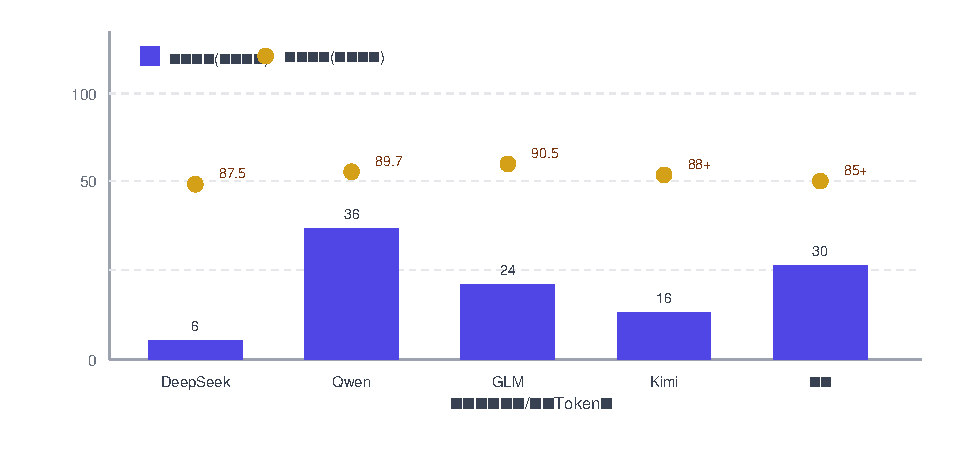
\includegraphics[width=0.92\linewidth]{figures/fig-di-si-shi-er-zhang-1}
\\[2pt]\small 圖 4：五款模型之價格與性能對比（價愈低愈好，分愈高愈好）
\end{center}

\booksection{三、模型選擇決策框架}

既識諸模型之特點，如何為己之專案擇模型？此授君一套「四問決策法」——答四問，即得鎖定至宜君之模型。

汝之項目於國內抑國際部署？

國內 選國產模型

|

國際 可選海外模型

核心任務為編程抑其他？

編程 Claude 或 DeepSeek

|

其他 繼續判斷

須超長上下文(>50萬Token)？

須 Gemini 或 Kimi

|

不須 繼續判斷

預算敏感嗎？

敏感 DeepSeek 或 Qwen-turbo

|

不敏感 GPT-5.6 或 Claude

\begin{center}\small\color{gray}圖 5：大模型選擇四問決策法\end{center}

\begin{tcbinfo}{小貼士：組合策略}
此決策法非教條——諸多場景需組合用多模型。一常見組合策略：以 DeepSeek 或 Qwen 為日常開發（成本低、中文佳），以 Claude 為關鍵架構設計（推理強、幻覺低），以 Gemini 為多模態分析（圖片影片處理）。按需切換模型，而非「一模型用至終」。

\end{tcbinfo}

\booksection{四、API 調用入門：從零接入大模型}

諸多 AI 編程教程惟教對話界面之用，然真「AI 編程」——使君之應用調用大模型——須經 API。API（Application Programming Interface，應用程序編程接口）者，程序之間通信之協議也。經 API，君之代碼可如調用一函數然，調用大模型之能。

\booksubsection{何謂 Token}

未解 API 之先，必先明「Token」之概念。Token 者，大模型計費之基本單位也，可解為「AI 閱讀與寫作之單位」。一 Token 約當：英文 0.75 詞（4 字符），中文 0.5-1 漢字。1000 字中文之文本，約耗 1500-2000 Token。

Token 非字數，亦非字符數。大模型用專門分詞器（Tokenizer）切文本為 Token。同詞於不同模型 Token 之數或異——如「人工智能」於 GPT 或為 3 Token，於 DeepSeek 或為 2。多數模型之 API 返實際消耗 Token 之數，君可於 API 回應中察之。

\begin{tcbinfo}{Token 成本速估}
100 萬字中文約當 150 萬 Token。以 DeepSeek V4 Flash 處理 100 萬字輸入 + 100 萬字輸出，成本約 0.42 美元（約 3 元人民幣）；以 Claude Fable 5 處理同量，成本約 60 美元（約 434 元人民幣）。此故模型之擇直接影響君專案之成本也。

\end{tcbinfo}

\booksubsection{獲取 API Key}

用大模型 API 之首步乃獲 API Key——驗證身份之密鑰也。每模型提供商各有其 API 平臺，君須註冊帳號並創建 API Key。以下乃主流模型 API 平臺入口與獲取流程：

\begin{center}
\begin{tabularx}{\linewidth}{|X|X|X|X|}
\hline
\textbf{模型} & \textbf{API 平臺} & \textbf{獲取流程} & \textbf{免費額度} \tabularnewline
\hline
DeepSeek & platform.deepseek.com & 註冊 實名認證 創建 API Key & 新用戶贈額度 \tabularnewline
通義千問 & bailian.aliyun.com（百煉平臺） & 阿里雲帳號登入 開通服務 創建 Key & 新用戶免費試用 \tabularnewline
智譜GLM & open.bigmodel.cn & 註冊 實名認證 創建 API Key & 新用戶贈額度 \tabularnewline
Kimi & platform.moonshot.cn & 註冊 實名認證 創建 API Key & 免費額度有限 \tabularnewline
豆包 & volcengine.com（火山引擎） & 註冊 開通方舟 創建 API Key & 註冊贈大量 Token \tabularnewline
OpenAI GPT & platform.openai.com & 註冊 綁定信用卡 創建 API Key & 無免費額度（須付費） \tabularnewline
Anthropic Claude & console.anthropic.com & 註冊 綁卡 創建 API Key & 新用戶少量額度 \tabularnewline
\hline
\end{tabularx}
\end{center}

\begin{center}\small\color{gray}主流模型 API 平臺及 Key 獲取之法（2026 年 8 月）\end{center}

\textbf{安全提示：API Key = 錢囊密碼}\par

API Key 同於君錢囊之密碼——凡得 Key 者皆可君之額度調用模型。故：永勿書 API Key 於代碼中（以環境變數管理之）；永勿以含 Key 之代碼提交於公開之 Git 倉庫；永勿於社羣媒體分享含 Key 之截圖。若 Key 洩露，即於平臺刪之而重新創建。

\booksubsection{首次 API 調用}

既獲 API Key，君可任何編程語言調用大模型 API。下以 Python 示至簡之調用——向 DeepSeek 發送一訊並取其覆。

\begin{lstlisting}[language=Python]
# 安裝SDK：pip install openai
# DeepSeek兼容OpenAI SDK格式，可直接用
from openai import OpenAI
import os

# 1. 建客戶端（API Key從環境變量讀取）
client = OpenAI(
    api_key=os.environ.get("DEEPSEEK_API_KEY"),
    base_url="https://api.deepseek.com"
)

# 2. 發送請求
response = client.chat.completions.create(
    model="deepseek-chat",  # 指定模型
    messages=[
        {"role": "system", "content": "汝乃Python編程之助。"},
        {"role": "user", "content": "寫一個快速排序函數。"}
    ]
)

# 3. 取回覆
print(response.choices[0].message.content)

# 4. 觀Token之耗
print(f"輸入Token: {response.usage.prompt_tokens}")
print(f"輸出Token: {response.usage.completion_tokens}")
print(f"總Token: {response.usage.total_tokens}")
\end{lstlisting}

此代碼核心邏輯：創建客戶端（攜 API Key 與模型之址） 構造訊息列表（system 設角色，user 為用戶輸入） 發送請求 獲取回覆。此式幾遍用於兼容 OpenAI 格式之模型——只需換 api\_key 與 base\_url 即可切換模型。此故諸多國產模型擇兼容 OpenAI SDK 格式：開發者只需改兩行代碼即切換模型，遷移成本至低。

下乃切換至他模型之代碼之異——注意只需改兩行：

\begin{lstlisting}[language=Python]
# DeepSeek
client = OpenAI(
    api_key=os.environ.get("DEEPSEEK_API_KEY"),
    base_url="https://api.deepseek.com"
)
# model="deepseek-chat"

# 通義千問（百鍊平臺）
client = OpenAI(
    api_key=os.environ.get("DASHSCOPE_API_KEY"),
    base_url="https://dashscope.aliyuncs.com/compatible-mode/v1"
)
# model="qwen-plus"

# 智譜GLM
client = OpenAI(
    api_key=os.environ.get("GLM_API_KEY"),
    base_url="https://open.bigmodel.cn/api/paas/v4"
)
# model="glm-4"

# OpenAI GPT
client = OpenAI(
    api_key=os.environ.get("OPENAI_API_KEY"),
    # base_url用默認值即可
)
# model="gpt-5.6-terra"
\end{lstlisting}

\booksubsection{流式回應處理}

實用之中，君常不欲待 AI 寫完所有內容方一次示之——為令用戶待之過久。流式回應（Streaming）可使君於 AI 生成之同時逐字顯示，大增用戶體驗。如打字機然，字一一蹦出，用戶之感全然不同也。

\begin{lstlisting}[language=Python]
# 流式之應：逐字而輸
stream = client.chat.completions.create(
    model="deepseek-chat",
    messages=[
        {"role": "user", "content": "著Python冒泡排序之教程"}
    ],
    stream=True  # 開啓流式響應
)

# 逐塊接收並打印
for chunk in stream:
    if chunk.choices[0].delta.content is not None:
        print(chunk.choices[0].delta.content, end="", flush=True)
# 輸出如打字機然，逐字而顯
\end{lstlisting}

\booksection{五、Token Plan 購買指南}

多數模型提供商有二計費之法：按量計費（Pay-as-you-go）與套餐訂閱（Token Plan / Subscription）。明此二法之別，可助君大降使用之成本。

\booksubsection{按量計費與套餐訂閱}

\begin{center}
\begin{tabularx}{\linewidth}{|X|X|X|}
\hline
\textbf{維度} & \textbf{按量計費（Pay-as-you-go）} & \textbf{套餐訂閱（Subscription）} \tabularnewline
\hline
計費方式 & 用幾許 Token 付幾許錢 & 預付固定費用，獲得額度 \tabularnewline
適合場景 & 使用量不穩、偶爾調用 & 使用量穩、高頻調用 \tabularnewline
價格優勢 & 標準價 & 較按量低 20\%-50\% \tabularnewline
靈活性 & 隨時可用，無須承諾 & 須預付，額度過期或作廢 \tabularnewline
超額處理 & 自動按量計費 & 超出額度後轉為按量計費 \tabularnewline
代表平臺 & 各模型官方API平臺 & OpenAI Plus/Pro, Claude Pro, Cursor Pro \tabularnewline
\hline
\end{tabularx}
\end{center}

\begin{center}\small\color{gray}二計費方式之對比\end{center}

初學者宜自按量計費始——不必預付費用，用幾許花幾許。月使用量既穩於一水平（如每月逾 50 元），乃考慮切換至套餐訂閱以得更低單價。

\booksubsection{主流訂閱套餐一覽}

\begin{center}
\begin{tabularx}{\linewidth}{|X|X|X|X|}
\hline
\textbf{套餐} & \textbf{月費} & \textbf{所含內容} & \textbf{適合人羣} \tabularnewline
\hline
ChatGPT Free & 免費 & GPT-5.6 Luna 無限文本對話 & 零基礎體驗 \tabularnewline
ChatGPT Plus & US\$20/月 & GPT-5.6 Sol、圖像生成、資料分析、插件訪問 & 中度使用戶 \tabularnewline
ChatGPT Pro & US\$200/月 & 無限制用所有模型、優先訪新功能 & 重度專業用戶 \tabularnewline
Claude Free & 免費 & 有限次數 Claude 對話 & 零基礎體驗 \tabularnewline
Claude Pro & US\$20/月 & 無限制 Claude 使用、優先訪新模型 & 編程開發者 \tabularnewline
Cursor Free & 免費 & 有限次數 AI 補全與對話 & 初學者體驗 \tabularnewline
Cursor Pro & US\$20/月 & 無限 AI 補全、500次/月高級請求 & 日常開發者 \tabularnewline
Cursor Business & US\$40/月/人 & 團隊協作、管理後臺、隱私模式 & 團隊使用 \tabularnewline
\hline
\end{tabularx}
\end{center}

\begin{center}\small\color{gray}主流 AI 工具訂閱套餐（2026 年 8 月）\end{center}

國內模型訂閱之方案略異。DeepSeek 主按量計費，無月度訂閱套餐——君儲值後按實際使用量扣費。通義千問於百煉平臺供預付費資源包（購一定量之 Token 額度，享折扣價）。豆包於火山引擎亦有相類預付費方案。於國內開發者，至經濟之組合通常為：DeepSeek 按量計費（日常開發）+ 豆包免費額度（體驗測試）。

\booksubsection{API 聚合平臺}

若君需同時用多模型，API 聚合平臺乃省心之選。聚合平臺供一統一之 API Key，君即得調用全球數十種模型，毋須於各平臺分別註冊。

\begin{center}
\begin{tabularx}{\linewidth}{|X|X|X|X|}
\hline
\textbf{平臺} & \textbf{特點} & \textbf{價格優勢} & \textbf{適合場景} \tabularnewline
\hline
OpenRouter (openrouter.ai) & 海外聚合平臺，一 Key 調用全球模型 & 價格透明，支援實時比價 & 需靈活切換多個海外模型 \tabularnewline
SiliconFlow (siliconflow.cn) & 國內聚合平臺，供多種國產模型API & 較官方低 20\%-30\% & 國內開發者，多模型比價 \tabularnewline
Azure OpenAI（微軟代理） & 微軟 Azure 代理之 OpenAI API & Batch API 可打5折 & 企業級 OpenAI 調用，大批量異步任務 \tabularnewline
百度千帆（qianfan.baidubce.com） & 百度 AI 雲平臺，供文心等模型 & 新用戶贈額度 & 百度生態用戶 \tabularnewline
\hline
\end{tabularx}
\end{center}

\begin{center}\small\color{gray}主流 API 聚合平臺（2026 年 8 月）\end{center}

\textbf{避坑提醒：勿購「共享 Key」}\par

勿於淘寶、閒魚等平臺購所謂「共享 API Key」——此等 Key 通常來路不明，或隨時被封號，且有資料洩露之險。恆經官方平臺或正規聚合平臺獲取 API Key。

\booksubsection{成本優化策略}

擇模型得當僅為首步，如何「用得省錢」亦同要。下乃數條經實踐驗證之成本優化策略：

\begin{enumerate}
  \item 善用緩存命中。諸多模型供「緩存」功能——君之請求若含之前已處理之內容（如系統提示詞），此部分僅以至低價格計費。DeepSeek 緩存命中之價僅為常價之 1/60。置固定之系統提示於訊息列表之首，可極大化緩存命中。
  \item 分級路由——以廉價模型處理簡單任務，貴模型處理複雜任務。如以 DeepSeek V4 Flash 為文本分類（輸出 2 元/百萬 Token），以 Claude 為架構設計（輸出 181 元/百萬 Token）。一專案中 80\% 之調用可用廉價模型。
  \item 限制輸出長度。API 按輸出 Token 計費，輸出愈長愈貴。於不需長篇大論之場景，設 max\_tokens 參數以限輸出長度，免 AI「廢話過多」。
  \item 以 Batch API 處理非實時任務。若君有大量不需即時回應之任務（如批量資料標註、文檔摘要），用 Batch API 可享 50\% 折扣。OpenAI 與 Azure 皆供此功能。
  \item 監察 Token 用量。多數 API 平臺供用量統計面板。定期察用量之分佈，尋耗 Token 至多之調用，因之優化。一小小 Prompt 之調整（如改「請詳解」為「請以 3 句解之」）可省 50\% 之 Token。
\end{enumerate}

\begin{center}
\begin{tabularx}{\linewidth}{|X|X|X|X|}
\hline
\textbf{優化策略} & \textbf{節省幅度} & \textbf{施行難度} & \textbf{說明} \tabularnewline
\hline
緩存命中 & 至高98\% & 低 & 置固定內容於訊息之首 \tabularnewline
分級路由 & 50\%-80\% & 中 & 簡單任務用廉價模型 \tabularnewline
限制輸出長度 & 30\%-60\% & 低 & 設 max\_tokens 參數 \tabularnewline
Batch API & 50\% & 低 & 非實時任務用批處理 \tabularnewline
Prompt優化 & 20\%-50\% & 中 & 精簡 Prompt，減少冗餘 \tabularnewline
\hline
\end{tabularx}
\end{center}

\begin{center}\small\color{gray}成本優化策略及效果（2026 年 8 月）\end{center}

\booksection{六、實戰：於專案中接入大模型 API}

請以一完整實戰終本章——創一「AI 摘要生成器」：用戶輸入一段長文本，調用大模型 API 生成摘要。此實戰將示 API 調用之完整流程：環境配置、API 調用、錯誤處理、成本控制。

\begin{lstlisting}[language=Python]
# ai_summarizer.py - AI摘要生成器
import os
from openai import OpenAI

# 1. 配置（API Key從環境變量讀取，絕不硬編碼）
client = OpenAI(
    api_key=os.environ.get("DEEPSEEK_API_KEY"),
    base_url="https://api.deepseek.com"
)

def summarize(text: str, max_length: int = 200) -> dict:
    """生成文本摘要

    Args:
        text: 要摘要之原文
        max_length: 摘要最大長度（Token數）

    Returns:
        dict: 包含摘要與Token消耗信息
    """
    try:
        response = client.chat.completions.create(
            model="deepseek-chat",
            messages=[
                {
                    "role": "system",
                    "content": "汝為一個摘要生成器。"
                               "請用簡潔之中文總結用戶提供之文本。"
                               "摘要不超過3句話。"
                },
                {
                    "role": "user",
                    "content": f"請摘要以下文本:\n\n{text}"
                }
            ],
            max_tokens=max_length,  # 限制輸出長度
            temperature=0.3  # 低溫度=更穩定
        )

        return {
            "success": True,
            "summary": response.choices[0].message.content,
            "input_tokens": response.usage.prompt_tokens,
            "output_tokens": response.usage.completion_tokens,
            "total_tokens": response.usage.total_tokens
        }

    except Exception as e:
        return {
            "success": False,
            "error": str(e)
        }

# 2. 使用示例
if __name__ == "__main__":
    long_text = """
    （粘貼一段長文本...）
    """

    result = summarize(long_text)

    if result["success"]:
        print(f"摘要: {result['summary']}")
        print(f"消耗Token: {result['total_tokens']}")
        # 估算成本：DeepSeek V4 Flash
        cost = result['total_tokens'] * 0.000004  # 約0.4分/千Token
        print(f"預估成本: {cost:.4f}元")
    else:
        print(f"出錯了: {result['error']}")
\end{lstlisting}

此代碼現 API 調用數項最佳實踐：API Key 經環境變數讀取，絕不硬編於代碼；函數有明晰文檔與型別提示；設 max\_tokens 限輸出長度；temperature 設低值（0.3）以得更穩輸出；有完整錯誤處理；返 Token 消耗之訊以追成本。君以 AI 作此代碼時，可告以此求——彼全然能助君實現。

本章之終極啟示：模型者，"彈藥"也；方法論者，"戰術"也。彈藥之良者可使戰鬥愈順，然戰術不善，彈藥雖美亦不能勝。既悉各模型之性與 API 之法，汝便握一充足之"彈藥庫"——然此仗如何打，終賴前數章所授之思維方法論。

\begin{tcbpractice}{來動手：跑通君首次 API 調用}
註冊一國產模型平臺（薦 DeepSeek 或智譜，皆贈新用戶額度），創建 API Key，書之於系統環境變數（而非代碼中！），乃運行上「首次 API 調用」之代碼。見 AI 回覆打印而出之刻，君已跨「用 AI」與「造 AI 應用」之界線矣。

\end{tcbpractice}

\begin{tcbsummary}{本章小結}
\begin{itemize}
  \item 國際三強：GPT-5.6（均衡全能）、Claude（編程天花板+幻覺率僅1\%）、Gemini（多模態之王+200萬上下文）
  \item 國產五強：DeepSeek V4（性價比之王，留意漲價公告）、Qwen3.7（企業級）、GLM-5.1（SWE國產第一）、Kimi K3（超長文本）、豆包（免費入門）
  \item 四問決策法：部署何地？編程抑其他？超長上下文？預算敏感乎？
  \item Token 為計費單位：中文 1 字約 1.5-2 Token；100萬字約150萬Token
  \item API Key = 錢囊密碼：環境變數管理，絕不硬編、不上傳 Git
  \item 國產模型普遍兼容 OpenAI SDK：換模型只需改 api\_key 與 base\_url 兩行
  \item 省錢五招：緩存命中、分級路由、限制輸出、Batch API、監察用量
\end{itemize}

\end{tcbsummary}
